% !TeX encoding = UTF-8
% !TeX spellcheck = en_US

\chapter{Fundamentals of Graph Transformations}
\label{fundamentals}
This chapter introduces the formal definitions for graph transformations based on category theory.
The definitions are based on Ehrig et al. \cite[pp. 21-47 and pp. 65-71]{FundamentalsOfAlgebraicGT} in a slightly different notation used in the lecture ``Fundamentals of Model-Driven Engineering'' by Anthony Anjorin.

\newcommand{\st}{.~}
\newcommand{\then}{\textbf{\,;\,}}
\newcommand{\gap}{\medskip \noindent}

\newcommand{\Graphs}{\textbf{Graphs}}
\newcommand{\TGraphs}{\textbf{TGraphs}}

% !TeX encoding = UTF-8
% !TeX spellcheck = en_US

\tikzset{
	defpicture/.style = {
		auto,
		node distance = 2cm,
		arrow/.style = {
			draw,
			->,
			shorten >=2pt,
		}
	},
	defnode/.style = {
		circle,
		draw = black
	},
	def1/.style = {
		text = red
	},
	def1-arrow/.style = {
		draw = red
	},
	def2/.style = {
		text = blue
	},
	def2-arrow/.style = {
		draw = blue
	}
}

% !TeX encoding = UTF-8
% !TeX spellcheck = en_US

\tikzset{
	tgraph/.style = {
		node distance = 0.5cm
	},
	tnode/.style = {
		fill = blue!10,
		inner sep = 3pt
	},
	tedge/.style = {
		draw = blue!50,
		thick,
		->
	},
	dlabel/.style = {
		inner sep = 1pt
	},
	dnode/.style = {
		draw = orange,
		thick,
		inner sep = 8pt
	},
	dedge/.style = {
		draw = orange,
		thick,
		->
	}
}


\section{Typed Graphs}
\label{fundamentals-typed-graphs}
Our models are attributed typed graphs.
Typed graphs are formally introduced in the following, while attributes are not formalized in this thesis.
The interested reader is referred to \cite{AttributedGraphTransformationViaRuleSchemata} or \cite{ComplexAttributeManipulationInTGGs} for a formalization of attributed graphs.

\begin{definition}[Category]
	\label{def:category}%
	A category $\mathbf{C} = (Ob, Arr, \then , id)$ consists of:
	\begin{itemize}
		\item a class $Ob$ of \emph{objects},
		\item for each pair of objects $A, B \in Ob$, a class $Arr_{(A, B)}$ of \emph{arrows},\\ where $f \in Arr_{(A,B)}$ is denoted by $f: A \rightarrow B$,
		\item for all objects $A, B, C \in Ob$,  a binary operation (for composing arrows):\\ 
		$\then: Arr_{(A,B)} \times Arr_{(B,C)} \rightarrow Arr_{(A,C)}$,
		\item for each object $A \in Ob$, an identity arrow $id_A: A \rightarrow A$,
	\end{itemize}
	such that the following conditions hold:
	\begin{itemize}
		\item Associativity.\\ $\forall A,B,C,D \in Ob\st \forall f: A \rightarrow B, g: B \rightarrow C, h: C \rightarrow D\st f \then (g \then h) = (f \then g) \then h$.
		\item Identity.\\ $\forall A, B \in Ob\st \forall f: A \rightarrow B\st (id_A \then f = f) \wedge (f \then id_B = f)$.
	\end{itemize}
\end{definition}

\noindent
In general, a category is a mathematical structure which has objects and morphisms.
A monomorphic arrow corresponds to an injective function.

\begin{definition}[Monomorphism]
	\label{def:monomorphism}%
	Let $\mathbf{C} = (Ob, Arr, \then , id)$ be a category.

	\gap
	An arrow \textcolor{red}{$f : X \rightarrow Y$} is monomorphic, iff 
	\[
		\forall\, g: Z \rightarrow X~ \forall\, h: Z \rightarrow X~ [(h;f = g;f) \Rightarrow (g = h)].
	\]
\end{definition}

\begin{figure}[h!]
	\centering
	\begin{tikzpicture}[defpicture]
	\node (Z) {$Z$};
	\node[def1, right of = Z] (X) {$X$};
	\node[def1, right of = X] (Y) {$Y$};

	\begin{scope}[every path/.style = arrow]
		\path (Z.20) to[bend left] node[above] {g} (X.160);
		\path (Z.340) to[bend right] node[below] {h} (X.200);
		\path[def1-arrow] (X) to node[def1] {f} (Y);
	\end{scope}
\end{tikzpicture}

	\caption{Monomorphism}
	\label{fig:monomorphism}
\end{figure}

\begin{definition}[Graphs and Graph Morphisms]
	\label{def:graphs}%
	A \emph{graph} \textcolor{red}{$G = (V, E, src, trg)$} consists of a set \textcolor{red}{$V$} of nodes (vertices), a set \textcolor{red}{$E$} of edges, and two functions \textcolor{red}{$src, trg: E \rightarrow V$} that assign each edge a source node and a target node, respectively.

	\gap
	Given graphs $G = (V, E,src,trg)$ and $G' = (V', E', src', trg')$, a \emph{graph morphism} \textcolor{blue}{$f: G \rightarrow G'$} consists of two functions
	\textcolor{blue}{$f_V: V \rightarrow V'$}
	and \textcolor{blue}{$f_E: E \rightarrow E'$}
	such that $src \then f_V = f_E \then src'$ and $trg \then f_V  = f_E \then trg'$.

	\gap
	$\Graphs = (Ob_{Graphs}, Arr_{Graphs}, \then_{Graphs}, id_{Graphs})$ consists of:
	\begin{itemize}
		\item graphs $Ob_{Graphs}$,
		\item graph morphisms $Arr_{Graphs}$,
		\item for $G, G', G'' \in Ob_{Graphs}$, $f =  G \rightarrow G'$, $g = G' \rightarrow G'' \in Arr_{Graphs}$, 
		$\then_{Graphs} (f,g) $ is defined as $f \then_{Graphs}~g := (f_V \then g_V, f_E \then g_E)$, 
		\item for $G = (V, E, src,trg) \in Ob_{Graphs}$,
		$id_G: G \rightarrow G$ is defined as $id_G := (id_V, id_E)$.
	\end{itemize}
\end{definition}

\begin{figure}[h!]
	\centering
	\begin{tikzpicture}[defpicture]
	\node[def1] (E) {$E$};
	\node[below of = E] (E') {$E'$};
	\node[def1, right of = E] (V) {$V$};
	\node[below of = V] (V') {$V'$};
	\node[def1, right = 1.5cm of V] (G) {$G = (E, V, src, trg)$};
	\node[below of = G] (G') {$G' = (E', V', src', trg')$};

	\begin{scope}[every path/.style = arrow]
		\path[def1-arrow] (E.20) to[bend left] node[def1, above] {src} (V.160);
		\path[def1-arrow] (E.340) to[bend right] node[def1, below] {trg} (V.200);

		\path[def2-arrow] (E) to node[def2, left] {$f_E$} (E');
		\path[def2-arrow] (V) to node[def2] {$f_V$} (V');

		\path (E'.20) to[bend left] node[above] {src'} (V'.160);
		\path (E'.340) to[bend right] node[below] {trg'} (V'.200);

		\path[def2-arrow] (G) to node[def2] {$f = (f_V, f_E)$} (G');
	\end{scope}
\end{tikzpicture}

	\caption{Graph Morphism}
	\label{fig:graph-morphism}
\end{figure}

\begin{definition}[Typed Graphs and Typed Graph Morphisms]
	\label{def:typed-graphs}%
	A \emph{type graph} is a distinguished graph $TG = (V_{TG}, E_{TG}, src_{TG}, trg_{TG})$.

	\gap
	A \emph{typed graph} is a pair $\hat{G} = (G, type)$ of a graph $G$ together with a graph morphism \textcolor{red}{$type: G \rightarrow TG$}.

	\gap
	Given typed graphs $\hat{G} = (G, type)$ and $\hat{G}' = (G', type')$, a \emph{typed graph morphism} $f: \hat{G} \rightarrow \hat{G}'$ is a graph morphism \textcolor{blue}{$f: G \rightarrow G'$} such that $f \then type' = type$.

	\gap
	$\TGraphs = (Ob_{TGraphs}, Arr_{TGraphs}, \then_{TGraphs}, id_{TGraphs})$ consists of:
	\begin{itemize}
		\item typed graphs $Ob_{TGraphs}$,
		\item typed graph morphisms $Arr_{TGraphs}$,
		\item $\then_{TGraphs} := \then_{Graphs}$,
		\item $id_{TGraphs} := id_{Graphs}$.
	\end{itemize}
\end{definition}

\noindent
Note that $\Graphs$ and $\TGraphs$ are categories according to Definition~\ref{def:category}.

\begin{figure}[h!]
	\centering
	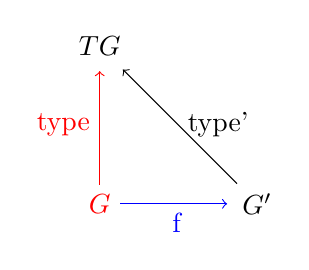
\begin{tikzpicture}[defpicture]
	\node (TG) {$TG$};
	\node[def1, below of = TG] (G) {$G$};
	\node[right of = G] (G') {$G'$};

	\begin{scope}[every path/.style = arrow]
		\path[def1-arrow] (G) to node[def1, left] {type} (TG);
		\path[def2-arrow] (G) to node[def2, below] {f} (G');
		\path (G') to node[right] {type'} (TG);
	\end{scope}
\end{tikzpicture}

	\caption{Typed Graph Morphism}
	\label{fig:typed-graph}
\end{figure}

\noindent
Figure~\ref{fig:example-type-graph} shows the type graph for the She Remembered Caterpillars meta-model introduced in Section~\ref{running-example}.
For clarity only the types used in the following examples are included.
A typed graph conforming to this type graph is shown in Figure~\ref{fig:example-typed-graph-instance}.
Each node is denoted by its name and its type, separated by a colon.
The edge labels are omitted in the graphs as they are comprehensible without ambiguity based on the types of their source and target node.

\begin{figure}[h!]
	\centering
	% !TeX encoding = UTF-8
% !TeX spellcheck = en_US

\begin{tikzpicture}
	\node[tnode] (game) {Game};
	\node[tnode, below = of game, xshift = -2cm] (character) {Character};
	\node[tnode, below = of game, xshift = 2cm] (platform) {Platform};

	\draw[tedge]
		(game)
		-- node[left, xshift = -0.2cm, yshift = 0.2cm] {characters}
		(character);
	\draw[tedge]
		(game)
		-- node[right, xshift = 0.2cm, yshift = 0.2cm] {platforms}
		(platform);
	\draw[tedge]
		(character)
		-- node[below] {standsOn}
		(platform);
	\draw[tedge]
		(platform.south)
		-- ++(0, -1)
		-- ++(1.25, 0)
		-- ++(0, 1.25)
		-- node[right, xshift = 0.3cm] {neighbors}
		(platform.east);
\end{tikzpicture}

	\caption{Type Graph for She Remembered Caterpillars (simplified)}
	\label{fig:example-type-graph}
\end{figure}

\begin{figure}[h!]
	\centering
	% !TeX encoding = UTF-8
% !TeX spellcheck = en_US

\begin{tikzpicture}
	\node[tnode] (g) {g: Game};
	\node[tnode, below = of g] (p) {p: Platform};
	\node[tnode, left = of p] (c) {c: Character};
	\node[tnode, right = of p] (q) {q: Platform};

	\draw[tedge] (g.west) -- (c);
	\draw[tedge] (c) -- (p);
	\draw[tedge] (g) -- (p);
	\draw[tedge] (g.east) -- (q);
	\draw[tedge] (p) -- (q);
\end{tikzpicture}

	\caption{Typed Graph Instance}
	\label{fig:example-typed-graph-instance}
\end{figure}

\section{Rule Applications}
\label{fundamentals-rule-applications}
A set of rules defines which model modifications are allowed in the graph transformation system.
The semantics of rule applications is given by the following definitions.

\begin{definition}[Pushouts]
	\label{def:pushouts}%
	Let $\mathbf{C} = (Ob, Arr, \then, id)$ be a category.

	\gap
	Given arrows \textcolor{red}{$r \in Arr: L \rightarrow R$} and \textcolor{red}{$m \in Arr: L \rightarrow G$}, a \emph{pushout} $(G', r', m')$ over $r$ and $m$ is defined by
	a \emph{pushout object} \textcolor{blue}{$G' \in Ob$}, and
	morphisms \textcolor{blue}{$r': G \rightarrow G'$}, \textcolor{blue}{$m': R \rightarrow G'$},
	where
	\begin{enumerate}
		\item the ``pushout square'' (Figure~\ref{fig:pushout}) commutes, \ie $r \then m' = m \then r'$,
		\item and the following universal property is fulfilled:\\
		$\forall\, G'' \in Ob~ \forall\, r'': G \rightarrow G''~ \forall\, m'': R \rightarrow G''$\\
		$[(r \then m'' = m \then r'') \Rightarrow (\exists!\, x: G' \rightarrow G''\, [(m' \then x = m'') \wedge (r' \then x = r'')])]$.
	\end{enumerate}
	The category $\mathbf{C}$ is said to \emph{have pushouts} if the pushout $(G', r', m')$ always exists. 
\end{definition}

\begin{figure}[h!]
	\centering
	\begin{tikzpicture}[defpicture]
	\node (L) {$L$};
	\node[right of = L] (R) {$R$};
	\node[below of = L] (G) {$G$};
	\node[def2, right of = G] (G') {$G'$};
	\node[right of = G', yshift = -2cm] (G'') {$G''$};

	\begin{scope}[every path/.style = arrow]
		\path[def1-arrow] (L) to node[def1] {$r$} (R);
		\path[def1-arrow] (L) to node[def1, left] {$m$} (G);
		\path[def2-arrow] (R) to node[def2] {$m'$} (G');
		\path[def2-arrow] (G) to node[def2, below] {$r'$} (G');
	\end{scope}

	\begin{scope}[every path/.style = arrow, dashed]
		\path (R) to[bend left] node {$m''$} (G'');
		\path (G) to[bend right] node {$r''$} (G'');
		\path (G') to node {$x$} (G'');
	\end{scope}
\end{tikzpicture}

	\caption{Pushout Diagram}
	\label{fig:pushout}
\end{figure}

\begin{figure}[h!]
	\centering
	% !TeX encoding = UTF-8
% !TeX spellcheck = en_US

\begin{tikzpicture}[remember picture]
	\node[dnode] (L) {
    	\begin{tikzpicture}[tgraph]
    	    \node[dlabel] (label) {$\mathbf{L}$};
	    	\node[tnode, below = 0.2cm of label] (g) {g: Game};
	    	\node[tnode, below = of g] (p) {p: Platform};
	    	\draw[tedge] (g) -- (p);
    	\end{tikzpicture}
  	};

  	\node[dnode, right = 1.2cm of L] (R) {
    	\begin{tikzpicture}[tgraph]
    		\node[dlabel] (label) {$\mathbf{R}$};
			\node[tnode, below = 0.2cm of label] (c) {c: Character};
			\node[tnode, below = of c] (g) {g: Game};
			\node[tnode, below = of g] (p) {p: Platform};
			\draw[tedge] (c)
				-- ++(-1.5,0)
				-- ++(0,-2.13)
				-- (p);
			\draw[tedge] (g) -- (c);
			\draw[tedge] (g) -- (p);
		\end{tikzpicture}
   	};

	\node[dnode, below = 2cm of L] (G) {	  	
		\begin{tikzpicture}[tgraph]
			\node[dlabel] (label) {$\mathbf{G}$};
		   	\node[tnode, below = 0.2cm of label] (g) {g: Game};
		   	\node[tnode, below = of g] (p) {p: Platform};
		   	\node[tnode, below = of p] (q) {q: Platform};
		   	\draw[tedge] (g) -- (p);
		   	\draw[tedge] (g.east)
			   	-- ++(0.6,0)
			   	-- ++(0,-2.13)
			   	-- (q.east);
		   	\draw[tedge] (p) -- (q);
	   	\end{tikzpicture}
	};

	\node[dnode, below = 1cm of R] (G') {
    	\begin{tikzpicture}[tgraph]
       	    \node[dlabel] (label) {$\mathbf{G'}$};
			\node[tnode, below = 0.2cm of label] (c) {c: Character};
			\node[tnode, below = of c] (g) {g: Game};
			\node[tnode, below = of g] (p) {p: Platform};
			\node[tnode, below = of p] (q) {q: Platform};
			\draw[tedge] (c)
				-- ++(-1.5,0)
				-- ++(0,-2.13)
				-- (p);
			\draw[tedge] (g) -- (c);
			\draw[tedge] (g) -- (p);
			\draw[tedge] (g.east)
				-- ++(0.6,0)
				-- ++(0,-2.13)
				-- (q.east);
			\draw[tedge] (p) -- (q);
		\end{tikzpicture}
   	};

	\draw[dedge] (L) -- node[above] {$r$} (R);
	\draw[dedge] (L) -- node[left] {$m$} (G);
	\draw[dedge] (R) -- node[right] {$m'$} (G');
	\draw[dedge] (G) -- node[below] {$r'$} (G');
\end{tikzpicture}

	\caption{Application of the Monotonic Rule \texttt{createCharacter}}
	\label{fig:example-monotonic-rule-application}
\end{figure}

\noindent
An application of a monotonic rule $r: L \rightarrow R$ requires finding a match in the host graph $G$ (\ie a monomorphic arrow $m: L \rightarrow G$) 
and constructing the resulting host graph $G'$ by applying the changes (\ie constructing the monomorphic arrow $m': R \rightarrow G'$) such that the constraints above are fulfilled.
$m'$ is called \emph{co-match}.
The universal property ensures that no elements are glued unnecessarily, while the commutation in the pushout square rejects all results $G'$ that do not glue enough.

Figure~\ref{fig:example-monotonic-rule-application} illustrates the pushout construction for a rule \texttt{createCharacter} which creates a new character and connects the character to a platform and the game.

\begin{definition}[Graph Transformation Rules]
	\label{def:graph-transformation-rules}%
	A \emph{(typed) graph transformation rule} \textcolor{red}{$L \stackrel{l}{\hookleftarrow} K \stackrel{r}{\hookrightarrow} R$} is a pair of monomorphic arrows in the category of (\textbf{T})\textbf{Graphs} with common ``gluing graph'' $K$. 
\end{definition}

\noindent
Monotonic rules can only handle creation, but not deletion of elements.
That is why the formalism $L \stackrel{l}{\hookleftarrow} K \stackrel{r}{\hookrightarrow} R$ is introduced in Definition~\ref{def:graph-transformation-rules}:
$l: K \hookrightarrow L$ describes the deletion, $r: K \hookrightarrow R$ the creation of elements.
The elements in $L \setminus K$ are deleted by the rule, the elements in $R \setminus K$ are created.
All elements in K remain unchanged.

In the following chapters of this thesis, graph transformation rules which do not have deleted or created elements (\ie $L \setminus K = \emptyset = R \setminus K$) are referred to as \textit{graph transformation patterns}.

\begin{definition}[Double-Pushout Graph Transformation Rule Application]
	\label{def:dpo-rule-application}%
	Given a (typed) graph transformation rule \textcolor{red}{$p = L \stackrel{l}{\hookleftarrow} K \stackrel{r}{\hookrightarrow} R$}, a \emph{direct derivation} with $p$ at a monomorphism $m: L \hookrightarrow G$, denoted by $G\stackrel{p@m}{\Longrightarrow}\textcolor{blue}{G'}$ (or $G\stackrel{p}{\Rightarrow}G'$, or $G \Rightarrow G'$), is given by the double-pushout (DPO) diagram below, where $(1)$ and $(2)$ are pushouts in the category \textbf{(T)Graphs}. 
\end{definition}

\begin{figure}[h!]
	\centering
	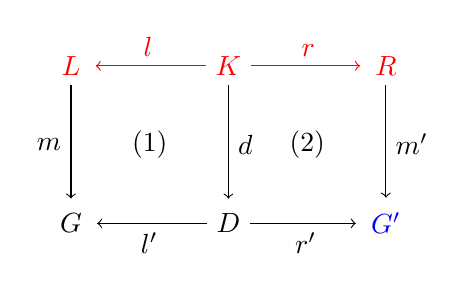
\begin{tikzpicture}[defpicture]
	\node[def1] (L) {$L$};
	\node[def1, right of = L] (K) {$K$};
	\node[def1, right of = K] (R) {$R$};

	\node[below of = L] (G) {$G$};
	\node[right of = G] (D) {$D$};
	\node[def2, right of = D] (G') {$G'$};

	\node[xshift = 1cm, yshift = -1cm] (s1) {(1)};
	\node[xshift = 3cm, yshift = -1cm] (s2) {(2)};

	\begin{scope}[every path/.style = arrow]
		\path[def1-arrow] (K) to node[def1, above] {$l$} (L);
		\path[def1-arrow] (K) to node[def1, above] {$r$} (R);

		\path (L) to node[left] {$m$} (G);
		\path (K) to node {$d$} (D);
		\path (R) to node {$m'$} (G');

		\path (D) to node[below] {$l'$} (G);
		\path (D) to node[below] {$r'$} (G');
	\end{scope}
\end{tikzpicture}

	\caption{Double-Pushout Diagram}
	\label{fig:double-pushout}
\end{figure}

\begin{definition}[Applicability of Graph Transformation Rules]
	\label{def:rule-applicability}%
	A (typed) graph transformation rule \textcolor{red}{$p = L \stackrel{l}{\hookleftarrow} K \stackrel{r}{\hookrightarrow} R$} is applicable to a (typed) graph $G$ via the  match $m: L \hookrightarrow G$,  if the pushout complement $D$ in the diagram below exists, such that (1) is a pushout in the category \textbf{(T)Graphs}.  
\end{definition}

\noindent
For the deletion part, taking the host graph as pushout object and completing square (1) leads to the pushout complement $D$.
After that the pushout is created in square (2) to obtain the resulting graph $G'$.

Figure~\ref{fig:example-dpo-rule-application} shows an application of the rule \texttt{moveCharacter} which deletes the edge between a character and its platform and creates a new edge between the character and another platform which must be neighboring to the previous one.
The construction of the pushout complement $D$ leads to the deletion of the edge between the character c and the platform p (so the rule is applicable according to Definition~\ref{def:rule-applicability}), while the pushout construction creates the new edge between the character c and the platform q, resulting in the graph $G'$.

\begin{figure}[h!]
	\centering
	% !TeX encoding = UTF-8
% !TeX spellcheck = en_US

\begin{tikzpicture}[remember picture]
	\node[dnode] (L) {
    	\begin{tikzpicture}[tgraph]
    		\node[dlabel] (label) {$\mathbf{L}$};
			\node[tnode, below = 0.2cm of label] (c) {c: Character};
			\node[tnode, below = of c] (p1) {p1: Platform};
			\node[tnode, below = of p1] (p2) {p2: Platform};
			\draw[tedge] (c) -- (p1);
			\draw[tedge] (p1) -- (p2);
		\end{tikzpicture}
  	};

	\node[dnode, right = 1.2cm of L] (K) {
    	\begin{tikzpicture}[tgraph]
    	    \node[dlabel] (label) {$\mathbf{K}$};
			\node[tnode, below = 0.2cm of label] (c) {c: Character};
			\node[tnode, below = of c] (p1) {p1: Platform};
			\node[tnode, below = of p1] (p2) {p2: Platform};
			\draw[tedge] (p1) -- (p2);
		\end{tikzpicture}
	};

  	\node[dnode, right = 1.2cm of K] (R) {
    	\begin{tikzpicture}[tgraph]
    	    \node[dlabel] (label) {$\mathbf{R}$};
			\node[tnode, below = 0.2cm of label] (c) {c: Character};
			\node[tnode, below = of c] (p1) {p1: Platform};
			\node[tnode, below = of p1] (p2) {p2: Platform};
			\draw[tedge] (c) 
				-- ++(-1.5,0)
				-- ++(0,-2.13)
				-- (p2);
			\draw[tedge] (p1) -- (p2);
		\end{tikzpicture}
   	};

	\node[dnode, below = 1cm of L] (G) {
    	\begin{tikzpicture}[tgraph]
    	    \node[dlabel] (label) {$\mathbf{G}$};
			\node[tnode, below = 0.2cm of label] (c) {c: Character};
			\node[tnode, below = of c] (g) {g: Game};
			\node[tnode, below = of g] (p) {p: Platform};
			\node[tnode, below = of p] (q) {q: Platform};
			\draw[tedge] (c)
				-- ++(-1.5,0)
				-- ++(0,-2.13)
				-- (p);
			\draw[tedge] (g) -- (c);
			\draw[tedge] (g) -- (p);
			\draw[tedge] (g.east)
				-- ++(0.6,0)
				-- ++(0,-2.13)
				-- (q.east);
			\draw[tedge] (p) -- (q);
		\end{tikzpicture}
	};

	\node[dnode, below = 1cm of K] (D) {
    	\begin{tikzpicture}[tgraph]
    	    \node[dlabel] (label) {$\mathbf{D}$};
			\node[tnode, below = 0.2cm of label] (c) {c: Character};
			\node[tnode, below = of c] (g) {g: Game};
			\node[tnode, below = of g] (p) {p: Platform};
			\node[tnode, below = of p] (q) {q: Platform};
			\draw[tedge] (g) -- (c);
			\draw[tedge] (g) -- (p);
			\draw[tedge] (g.east)
				-- ++(0.6,0)
				-- ++(0,-2.13)
				-- (q.east);
			\draw[tedge] (p) -- (q);
		\end{tikzpicture}
	};

	\node[dnode, below = 1cm of R] (G') {
    	\begin{tikzpicture}[tgraph]
    		\node[dlabel] (label) {$\mathbf{G'}$};
			\node[tnode, below = 0.2cm of label] (c) {c: Character};
			\node[tnode, below = of c] (g) {g: Game};
			\node[tnode, below = of g] (p) {p: Platform};
			\node[tnode, below = of p] (q) {q: Platform};
			\draw[tedge] (c)
				-- ++(-1.5,0)
				-- ++(0,-3.13)
				-- (q);
			\draw[tedge] (g) -- (c);
			\draw[tedge] (g) -- (p);
			\draw[tedge] (g.east)
				-- ++(0.6,0)
				-- ++(0,-2.13)
				-- (q.east);
			\draw[tedge] (p) -- (q);
		\end{tikzpicture}
   	};

	\draw[dedge] (K) -- node[above] {$l$} (L);
	\draw[dedge] (K) -- node[above] {$r$} (R);

	\draw[dedge] (L) -- node[left] {$m$} (G);
	\draw[dedge] (K) -- node[right] {$d$} (D);
 	\draw[dedge] (R) -- node[right] {$m'$} (G');

	\draw[dedge] (D) -- node[below] {$l'$} (G);
	\draw[dedge] (D) -- node[below] {$r'$} (G');
\end{tikzpicture}

	\caption{Application of the Graph Transformation Rule \texttt{moveCharacter}}
	\label{fig:example-dpo-rule-application}
\end{figure}

\begin{definition}[Dangling Edge Condition]
	\label{def:dangling-edge-condition}%
	Given a (typed) graph transformation rule $p = L \stackrel{l}{\hookleftarrow} K \stackrel{r}{\hookrightarrow} R$ and a match $m: L \hookrightarrow G$, the set of \emph{dangling points} (DP) is defined as:
	\[
		DP = \{ v \in V_L ~|~ \exists e \in (E_G \setminus m_E(E_L))~[\,(s_G(e) = m_V(v)) \vee (t_G(e) = m_V(v))\,] \}
	\]

	\gap
	The set of \emph{gluing points} (GP) is defined as $GP = l_V(V_K)$.

	\gap
	The \emph{Dangling Edge Condition} is fulfilled by $p$ and $m$ iff $DP \subseteq GP$.   
\end{definition}

\begin{theorem}[Existence and Uniqueness of Pushout Complements]
	\label{theorem:existence-and-uniqueness-of-pushout-complements}%
	Given a (typed) graph transformation rule $p = L \stackrel{l}{\hookleftarrow} K \stackrel{r}{\hookrightarrow} R$ and a match $m: L \hookrightarrow G$, the pushout complement $\{D, d: K \hookrightarrow D, l': D \hookrightarrow G\}$ of $l$ and $m$ exists and is unique up to isomorphism iff the dangling edge condition is fulfilled.  
\end{theorem}

\noindent
Dangling edges are edges whose source or target node is deleted during the application, without the edge itself is defined as a deleted edge by $l: K \hookrightarrow L$.
Such edges must not be left over after rule application, as they lead to an invalid graph -- that is why an approach to avoid dangling edges after rule application is necessary.
Theorem~\ref{theorem:existence-and-uniqueness-of-pushout-complements} states that a rule is applicable according to DPO if and only if there are no dangling edges.\footnote{see \cite[Fact 3.11, pp. 45-46]{FundamentalsOfAlgebraicGT} for a proof of Theorem~\ref{theorem:existence-and-uniqueness-of-pushout-complements}}
So dangling edges cannot be left over after rule application, as their existence prevents rule application.

Besides DPO rule application according to Definition~\ref{def:dpo-rule-application}, another pushout approach called \textit{single-pushout} (SPO) exists.\footnote{see \cite{HandbookOfGraphGrammars1997} for a formal definition of SPO}
SPO relaxes the strict precondition for rule application such that there may be dangling edges:
If there are dangling edges, the rule is still applicable and the dangling edges are deleted by the rule application.

\section{Application Conditions}
\label{fundamentals-application-conditions}
Application conditions can be used to define additional constraints for rule applications.
A rule with an application condition can only be applied if the rule is applicable according to the pushout approach (DPO as defined in Definition~\ref{def:rule-applicability} or SPO) and the application conditions are fulfilled.

\begin{definition}[Graph Condition]
	\label{def:graph-conditions}%
	Let  $\mathbf{C} = (Ob, Arr, \then, id)$ be a category.

	\gap
	A \emph{graph condition} over an object $L$ is a pair 
	\textcolor{red}{$gc = (p: L \rightarrow P, \{ c_i: P \rightarrow C_i ~|~ i \in I \})$}, for some index set $I$.

	\gap
	$L \in Ob$ is referred to as the \emph{context}, $p \in Arr$ the \emph{premise}, and $\{ c_i \in Arr ~|~ i \in I \}$ the \emph{conclusions} of the graph condition $gc$.  
\end{definition}

\begin{definition}[Satisfaction of Graph Conditions]
	\label{def:satisfaction-of-graph-conditions}%
	Let $\mathbf{C} = (Ob, Arr, \then , id)$ be a category, and $gc$ a graph condition over $L \in Ob$ for some index set $I$, i.e., \textcolor{red}{$gc = (p: L \rightarrow P, \{ c_i: P \rightarrow C_i ~|~ i \in I \})$}.

	\gap
	An arrow $m: L \rightarrow G$ \emph{satisfies} $gc$, denoted by $m \models gc$, iff\\ 
	\[
		\forall\, m_p: P \rightarrow G ~[(m = p \then m_p) \Rightarrow (\exists\, i \in I\, \exists\, m_{c_i}: C_i \rightarrow G ~[m_p = c_i \then m_{c_i}])],
	\]
	where $m_p, (m_{c_i})_{i \in I}$ are monomorphisms.
\end{definition}

\begin{figure}[h!]
	\centering
	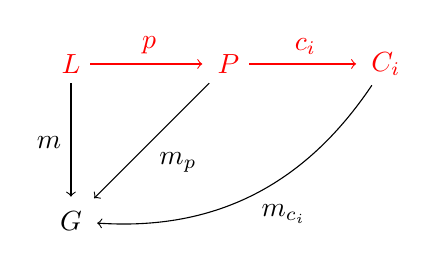
\begin{tikzpicture}[defpicture]
	\node[def1] (L) {$L$};
	\node[def1, right of = L] (P) {$P$};
	\node[def1, right of = P] (C) {$C_i$};
	\node[below of = L] (G) {$G$};

	\begin{scope}[every path/.style = arrow]
		\path[def1-arrow] (L) to node[def1, above] {$p$} (P);
		\path[def1-arrow] (P) to node[def1] {$c_i$} (C);

		\path (L) to node[left] {$m$} (G);
		\path (P) to node {$m_p$} (G);
		\path (C) to[bend left] node {$m_{c_i}$} (G);
	\end{scope}
\end{tikzpicture}

	\caption{Graph Condition}
	\label{fig:graph-condition}
\end{figure}

\noindent
There are two possibilities to satisfy a graph condition:
If there does not exist a monomorphic arrow $m_p: P \rightarrow G$, the condition is trivially satisfied (because the premise does not hold).
In addition, the graph condition is satisfied if there is at least one $i \in I$ for which a monomorphic arrow $m_{c_i}: C_i \rightarrow G$ exists (one of the conclusion is fulfilled).

Graph conditions can be combined via logical expressions using negation ($\neg$), conjunction ($\wedge$) and disjunction ($\vee$) as defined in Definition~\ref{def:complex-graph-conditions}.

\begin{definition}[Complex Graph Conditions]
	\label{def:complex-graph-conditions}
	$true$ is a complex graph condition.

	\gap
	A graph condition $gc$ is a complex graph condition.

	\gap
	$\neg c$ is a complex graph condition, where $c$ is a complex graph condition.

	\gap
	$\wedge_{j \in J}\, c_j$ is a complex graph condition, where $J$ is an index set and $(c_j)_{j \in J}$ are complex graph conditions.

	\gap
	$false$ is an abbreviation for $\neg true$.

	\gap
	$\vee_{j \in J}\, c_j$ is an abbreviation for $\neg (\wedge_{j \in J}\, \neg c_j)$.

	\gap
	$c \Rightarrow d$ is an abbreviation for $\neg c \vee d$.
\end{definition}

\begin{definition}[Satisfaction of Complex Graph Conditions]
	\label{def:satisfaction-of-complex-graph-conditions}%
	Let $\mathbf{C} = (Ob, Arr, \then , id)$ be a category, and $c$ a complex graph condition over $L \in Ob$.

	\gap
	An arrow $m \in Arr: L \rightarrow G$ \emph{satisfies} the complex graph condition $c$, denoted by $m \models c$, iff one of the following holds:
	\begin{itemize}
		\item $c = true$
		\item $c = gc$, $gc$ is a graph condition, and $m \models gc$
		\item $c = \neg c'$, and $m \not\models c'$ ($m$ does not satisfy $c'$)
		\item $c = \wedge_{j \in J}\, c_j$, and $\forall_{j \in J}\, [m \models c_j]$.  
	\end{itemize}
\end{definition}

\noindent
Given a rule $r: L \rightarrow R$, a graph condition using the left-hand side of the rule as context forms an application condition.
A rule is only applicable for a match $m: L \rightarrow G$ if the application conditions of the rule are satisfied.

\begin{definition}[Application Conditions]
	\label{def:application-conditions}%
	Let  $\mathbf{C} = (Ob, Arr, \then , id)$ be a category with pushouts.

	\gap
	Given a monotonic rule $r \in Arr: L \rightarrow R$, an \emph{application condition} $ac$ for $r$ is a graph condition \textcolor{red}{$(p: L \rightarrow P, \{ c_i: P \rightarrow C_i ~|~ i \in I \})$} over $L$.

	\gap
	A direct derivation $d = G \stackrel{r@m}{\Longrightarrow} G'$ with $r$ at match $m: L \rightarrow G$ satisfies $ac$, denoted by $d \models ac$, iff $m \models ac$ according to Definitions~\ref{def:satisfaction-of-graph-conditions} and~\ref{def:satisfaction-of-complex-graph-conditions}. 
\end{definition}

\begin{figure}[h!]
	\centering
	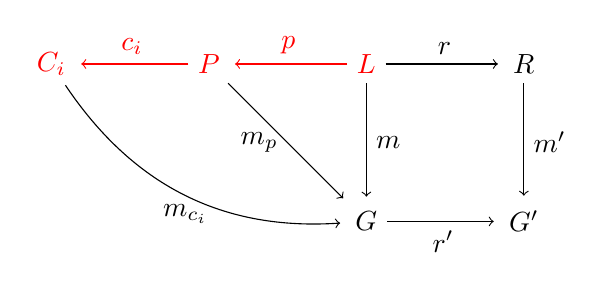
\begin{tikzpicture}[defpicture]
	\node[def1] (P) {$P$};
	\node[def1, right of = P] (L) {$L$};
	\node[right of = L] (R) {$R$};
	
	\node[def1, left of = P] (C) {$C_i$};

	\node[below of = L] (G) {$G$};
	\node[right of = G] (G') {$G'$};

	\begin{scope}[every path/.style = arrow]
		\path[def1-arrow] (L) to node[def1, above] {$p$} (P);
		\path (L) to node[above] {$r$} (R);

		\path (L) to node[right] {$m$} (G);
		\path (R) to node {$m'$} (G');
		\path (G) to node[below] {$r'$} (G');

		\path (P) to node[left] {$m_p$} (G);
		\path[def1-arrow] (P) to node[def1, above] {$c_i$} (C);
		\path (C) to[bend right] node[below] {$m_{c_i}$} (G);
	\end{scope}
\end{tikzpicture}

	\caption{Application Condition for Monotonic Rules}
	\label{fig:application-condition}
\end{figure}

\begin{definition}[Negative Application Conditions (NAC)]
	\label{def:nacs}%
	Let  $\mathbf{C} = (Ob, Arr, \then , id)$ be a category with pushouts.

	\gap
	Given a monotonic rule $r \in Arr: L \rightarrow R$, a \emph{negative application condition (NAC)} for $r$ is an application condition for $r$ of the form \textcolor{red}{$(n: L \rightarrow N, \{\})$}.
\end{definition}

\begin{figure}[h!]
	\centering
	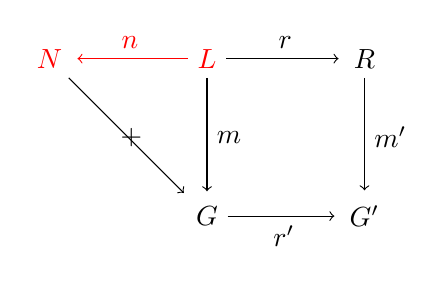
\begin{tikzpicture}[defpicture]
	\node[def1] (N) {$N$};
	\node[def1, right of = N] (L) {$L$};
	\node[right of = L] (R) {$R$};

	\node[below of = L] (G) {$G$};
	\node[right of = G] (G') {$G'$};

	\begin{scope}[every path/.style = arrow]
		\path[def1-arrow] (L) to node[def1, above] {$n$} (N);
		\path (L) to node[above] {$r$} (R);

		\path (L) to node[right] {$m$} (G);
		\path (R) to node {$m'$} (G');
		\path (G) to node[below] {$r'$} (G');

		\path (N) to node[left, xshift = 3mm] {$+$} (G);
	\end{scope}
\end{tikzpicture}

	\caption{Negative Application Condition for Monotonic Rules}
	\label{fig:nac}
\end{figure}

\noindent
A NAC is violated if and only if a premise $N$ exists as there are no conclusions, \ie the NAC is satisfied if there is no $N$ such that the arrow $N \rightarrow G$ can be constructed.

\begin{figure}[h!]
	\centering
	% !TeX encoding = UTF-8
% !TeX spellcheck = en_US

\begin{tikzpicture}[remember picture]
	\node[dnode] (N) {
		\begin{tikzpicture}[tgraph]
			\node[dlabel] (labelN) {$\mathbf{N}$};
			\node[tnode, below = 0.2cm of labelN] (p) {p: Platform};
			\node[tnode, below = of p] (c') {c$'$: Character};
			\draw[tedge] (c') -- (p);
		\end{tikzpicture}
	};

	\node[dnode, right = 1.2cm of N] (L) {
    	\begin{tikzpicture}[tgraph]
    		\node[dlabel] (labelL) {$\mathbf{L}$};
	    	\node[tnode, below = 0.2cm of labelL] (g) {g: Game};
	    	\node[tnode, below = of g] (p) {p: Platform};
	    	\draw[tedge] (g) -- (p);
    	\end{tikzpicture}
  	};

  	\node[dnode, right = 1.2cm of L] (R) {
    	\begin{tikzpicture}[tgraph]
    		\node[dlabel] (labelR) {$\mathbf{R}$};
			\node[tnode, below = 0.2cm of labelR] (c) {c: Character};
			\node[tnode, below = of c] (g) {g: Game};
			\node[tnode, below = of g] (p) {p: Platform};
			\draw[tedge] (c)
				-- ++(-1.5,0)
				-- ++(0,-2.13)
				-- (p);
			\draw[tedge] (g) -- (c);
			\draw[tedge] (g) -- (p);
		\end{tikzpicture}
   	};

	\node[dnode, below = 1.95cm of L] (G) {	  	
		\begin{tikzpicture}[tgraph]
			\node[dlabel] (labelG) {$\mathbf{G}$};
		   	\node[tnode, below = 0.2cm of labelG] (g) {g: Game};
		   	\node[tnode, below = of g] (p) {p: Platform};
		   	\node[tnode, below = of p] (q) {q: Platform};
		   	\draw[tedge] (g) -- (p);
		   	\draw[tedge] (g.east)
			   	-- ++(0.6,0)
			   	-- ++(0,-2.13)
			   	-- (q.east);
		   	\draw[tedge] (p) -- (q);
	   	\end{tikzpicture}
	};

	\node[dnode, below = 1cm of R] (G') {
    	\begin{tikzpicture}[tgraph]
    		\node[dlabel] (labelG') {$\mathbf{G'}$};
			\node[tnode, below = 0.2cm of labelG'] (c) {c: Character};
			\node[tnode, below = of c] (g) {g: Game};
			\node[tnode, below = of g] (p) {p: Platform};
			\node[tnode, below = of p] (q) {q: Platform};
			\draw[tedge] (c)
				-- ++(-1.5,0)
				-- ++(0,-2.11)
				-- (p);
			\draw[tedge] (g) -- (c);
			\draw[tedge] (g) -- (p);
			\draw[tedge] (g.east)
				-- ++(0.6,0)
				-- ++(0,-2.13)
				-- (q.east);
			\draw[tedge] (p) -- (q);
		\end{tikzpicture}
   	};

	\draw[dedge] (L) -- node[above] {$r$} (R);
	\draw[dedge] (L) -- node[left] {$m$} (G);
	\draw[dedge] (L) -- node[above] {$n$} (N);
	\draw[dedge] (N.south) -- node[color = orange, left, xshift = 3mm] {$+$} (G.west);
	\draw[dedge] (R) -- node[right] {$m'$} (G');
	\draw[dedge] (G) -- node[below] {$r'$} (G');
\end{tikzpicture}

	\caption{Negative Application Condition for the Monotonic Rule \texttt{createCharacter}}
	\label{fig:example-nac}
\end{figure}

\noindent
Figure~\ref{fig:example-nac} shows an example NAC for the rule \texttt{createCharacter}.
The NAC ensures that there is no other character which stands already on the platform the new character is placed on. 
As the arrow $N \rightarrow G$ cannot be constructed, the rule is still applicable.
Note that a second rule application with the same match $m$ is not possible after the shown application to $G$ because the arrow $N \rightarrow G'$ ($G'$ from the first rule application is the new $G$ for the next rule application) can be constructed for the match choosing the platform p.
A new character could still be added if $m$ chooses platform q, \ie a the new character stands on q.

The definition of application conditions for monotonic rules $r: L \rightarrow R$ can be easily extended to graph transformation rules $p = L \hookleftarrow K \hookrightarrow R$ as only rule applicability is affected by the definition.
Figures~\ref{fig:application-condition-gt} and~\ref{fig:nac-gt} show the modified diagrams.

\begin{figure}[h!]
	\centering
	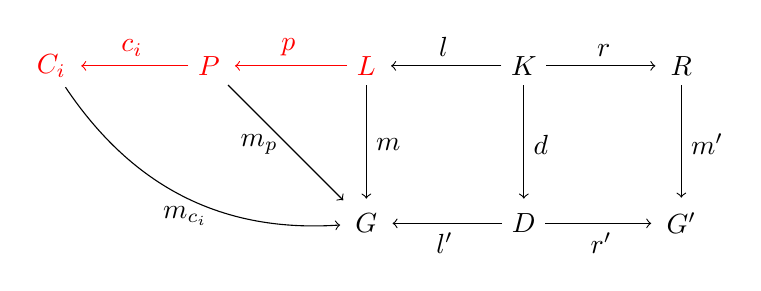
\begin{tikzpicture}[defpicture]
	\node[def1] (P) {$P$};
	\node[def1, right of = P] (L) {$L$};
	\node[right of = L] (K) {$K$};
	\node[right of = K] (R) {$R$};

	\node[def1, left of = P] (C) {$C_i$};

	\node[below of = L] (G) {$G$};
	\node[right of = G] (D) {$D$};
	\node[right of = D] (G') {$G'$};

	\begin{scope}[every path/.style = arrow]
		\path[def1-arrow] (L) to node[def1, above] {$p$} (P);

		\path (K) to node[above] {$l$} (L);
		\path (K) to node[above] {$r$} (R);

		\path (L) to node[right] {$m$} (G);
		\path (K) to node {$d$} (D);
		\path (R) to node {$m'$} (G');

		\path (D) to node[below] {$l'$} (G);
		\path (D) to node[below] {$r'$} (G');

		\path (P) to node[left] {$m_p$} (G);
		\path[def1-arrow] (P) to node[def1, above] {$c_i$} (C);
		\path (C) to[bend right] node[below] {$m_{c_i}$} (G);
	\end{scope}
\end{tikzpicture}

	\caption{Application Condition for Graph Transformation Rules}
	\label{fig:application-condition-gt}
\end{figure}

\begin{figure}[h!]
	\centering
	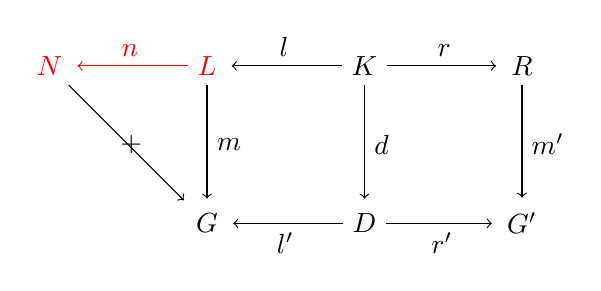
\begin{tikzpicture}[defpicture]
	\node[def1] (N) {$N$};
	\node[def1, right of = N] (L) {$L$};
	\node[right of = L] (K) {$K$};
	\node[right of = K] (R) {$R$};

	\node[below of = L] (G) {$G$};
	\node[right of = G] (D) {$D$};
	\node[right of = D] (G') {$G'$};

	\begin{scope}[every path/.style = arrow]
		\path[def1-arrow] (L) to node[def1, above] {$n$} (N);

		\path (K) to node[above] {$l$} (L);
		\path (K) to node[above] {$r$} (R);

		\path (L) to node[right] {$m$} (G);
		\path (K) to node {$d$} (D);
		\path (R) to node {$m'$} (G');

		\path (D) to node[below] {$l'$} (G);
		\path (D) to node[below] {$r'$} (G');

		\path (N) to node[left, xshift = 3mm] {$+$} (G);
	\end{scope}
\end{tikzpicture}

	\caption{Negative Application Condition for Graph Transformation Rules}
	\label{fig:nac-gt}
\end{figure}
